\documentclass[
	% sans,			% use sans-serif font
	% serif,			% use serif-font
	%mathsans,		% set mathtext to sans-serif
	%mathserif,		% set mathtext to serif
	%10pt,
	10pt,
	%12pt,
	t		% add text at the top border of slide
	%slidescentered,% center text on slide
	%draft,			% compile as draft version
	%handout,		% create handout file
	% notes,			% include nodes in slides
	%compress		% compress navigation bar
]{beamer}

\usetheme{lmtslides}
\usepackage{eso-pic}
\usepackage{graphicx}
% \usepackage[pdftex]{color}
\usepackage{times}
\usepackage[latin1]{inputenc}
\usepackage[T1]{fontenc}
\usepackage[amssymb]{SIunits}
\usepackage{amsmath,amssymb}
\usepackage{eurosym}
\usepackage{booktabs}
\usepackage{colortbl}
\usepackage{url}
\usepackage[absolute,overlay]{textpos}
\usepackage{graphicx}
\usepackage{mathtools}
\usepackage{pifont}% http://ctan.org/pkg/pifont
\usepackage{appendixnumberbeamer}
\usepackage{subcaption}
\usepackage{tikz}
\usepackage{pgfplots}
\usepackage{multimedia}
\usepackage{media9}
\addmediapath{figures/}



\usetikzlibrary{shapes.geometric, arrows}
\usetikzlibrary{positioning}
\usetikzlibrary{arrows}
\usetikzlibrary{calc}

\newcommand{\xmark}{\ding{55}}%
\newcommand{\cmark}{\ding{51}}%

\renewcommand{\footnoterule}{\vfill\kern -3pt  \kern 2.6pt}

\setbeamertemplate{caption}{\raggedright\insertcaption\par}
\setbeamertemplate{bibliography item}[online]
\graphicspath{{figures/}}

\setlang{en}		

% Supervisor: Univ.-Prof. Dr. Hans-Joachim Bungartz
% Advisors: Manish Kumar Mishra, M.Sc. (hons) &
% Samuel James Newcome, M.Sc.

% MODIFY THESE ACCORDINGLY! ---
\title{Algorithm Selection and Auto-Tuning in AutoPas}
\type{Sf} % (M/B/D/S)(f/m): (Master/Bachelor/Diplom/Studienarbeit)(final/midterm)
\author{Manuel Lerchner}
\email{manuel.lerchner@tum.de}
\advisorOne{Manish Kumar Mishra, M.Sc. (hons)}
\date{\today}
%------------------------------



\AtBeginSection[]
{
    \begin{frame}
        \frametitle{Table of Contents}
        \tableofcontents[currentsection,currentsubsection]
    \end{frame}
}

%%%%%%%%%%%%%%%%%%%%%%%%%%
\begin{document}

\maketitle

\setcounter{framenumber}{0}

\section{Introduction}

\begin{frame}{Software Challenges in Molecular Dynamics}
    \begin{itemize}
        \item Enormous numbers of particles
              \begin{itemize}
                  \item naively: $\mathcal{O}(N^2)$ interactions
              \end{itemize}
        \item Solution: highly optimized algorithms
              \begin{itemize}
                  \item Make full use of hardware
                  \item Smart data structures
              \end{itemize}
        \item Every millisecond counts
    \end{itemize}



    \begin{textblock*}{4.5cm}(7cm,5cm)
        \begin{center}
            \includegraphics[width=\textwidth]{figures/rayleigh_taylor_instability_3d.png}
        \end{center}
    \end{textblock*}



\end{frame}

\section{Algorithmic Trade-offs}

\begin{frame}
    \frametitle{Trade-off: Particle Containers}

    \begin{itemize}
        \item How to identify interacting particles?
        \item Short-range forces allow for cutoff radius $\rightarrow$ $\mathcal{O}(N)$ interactions
        \item Different implementations possible
    \end{itemize}

    \vspace{0.2cm}
    \begin{figure}
        \centering
        \includegraphics[width=0.75\textwidth]{figures/particle_containers.png}
        \caption{\small{
                \cite{SIAM_PP24}}}
    \end{figure}

\end{frame}


% \begin{frame}
%     \frametitle{}
%     \begin{itemize}
%         \item Shared memory traversals
%         \item Data layouts
%         \item Newton 3 optimization
%         \item $\dots$


%         \item Best choice depends on:
%               \begin{itemize}
%                   \item Hardware
%                   \item Scenario
%               \end{itemize}
%     \end{itemize}
% \end{frame}


\begin{frame}
    \frametitle{Many more difficult choices}
    \begin{itemize}
        \item No silver bullet!
        \item Hardware- and Scenario-dependent
    \end{itemize}
    \begin{center}


        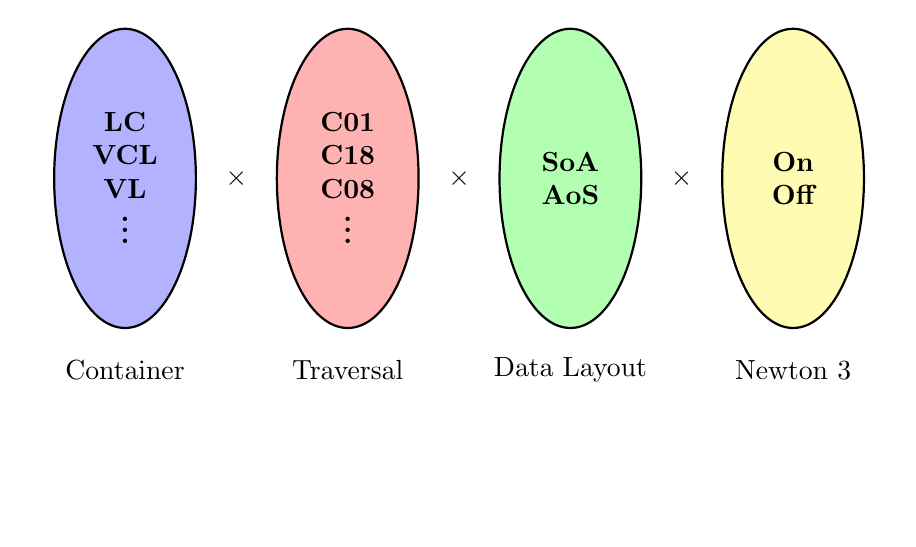
\begin{tikzpicture}[
                node distance=1cm,
                thick,
                every node/.style={
                        draw,
                        ellipse,
                        minimum width=1.8cm,
                        minimum height=3.8cm,
                        align=center
                    },
                textnode/.style={
                        draw=none,
                        align=center
                    }
            ]

            % Nodes with colors
            \node[fill=blue!30,font=\bfseries] (A) {LC\\VCL\\VL\\ \vdots};
            \node[fill=red!30, right=of A,font=\bfseries] (B) {C01\\C18\\C08\\ \vdots};
            \node[fill=green!30, right=of B,font=\bfseries] (C) {SoA\\AoS};
            \node[fill=yellow!30, right=of C,font=\bfseries] (D) {On\\Off};

            % Text underneath ellipses with matching colors
            \node[textnode, below=-1.4cm of A, ] (Atext) {Container};
            \node[textnode, below=-1.4cm of B, ] (Btext) {Traversal};
            \node[textnode, below=-1.4cm of C, ] (Ctext) {Data Layout};
            \node[textnode, below=-1.4cm of D, ] (Dtext) {Newton 3};

            % Crosses between the nodes
            \draw[->, draw=none] (A) -- (B) node[midway, draw=none] {$\times$};
            \draw[->, draw=none] (B) -- (C) node[midway, draw=none] {$\times$};
            \draw[->, draw=none] (C) -- (D) node[midway, draw=none] {$\times$};

        \end{tikzpicture}
    \end{center}


\end{frame}



\begin{frame}{Traditional MD Engines}


    \begin{textblock*}{3.5cm}(8.5cm,2.2cm)
        \includegraphics[width=3.5cm]{figures/gromacs-logo.png}
    \end{textblock*}
    \begin{textblock*}{3.5cm}(8.5cm,4cm)
        \includegraphics[width=3.5cm]{figures/lammps-logo.png}
    \end{textblock*}
    \begin{textblock*}{3cm}(8.5cm,5.3cm)
        \begin{center}

            \includegraphics[width=1.5cm]{figures/ls1-logo.png}
        \end{center}
    \end{textblock*}


    \begin{itemize}
        \item Based on a single container
        \item Performance through:
              \begin{itemize}
                  \item Very optimized code
                  \item Vectorization
              \end{itemize}
        \item Drawbacks:
              \begin{itemize}
                  \item Suboptimal for some scenarios
                  \item Require manual tuning
              \end{itemize}
    \end{itemize}

\end{frame}

\section{AutoPas Framework}

\begin{frame}
    \frametitle{What is AutoPas?}

    \begin{textblock*}{5cm}(9cm,1.8cm)
        \includegraphics[width=3cm]{figures/AutoPasLogo}
    \end{textblock*}

    \begin{itemize}
        \item Library for arbitrary N-body simulations
        \item Implements all algorithms
              \begin{itemize}
                  \item Modular
                  \item All\textup{\small*} configurations possible
              \end{itemize}
        \item Idea: AutoTuning
              \begin{itemize}
                  \item Finds optimal configuration
                  \item[$\rightarrow$] Thus optimal performance
              \end{itemize}
        \item Arbitrary user code
    \end{itemize}

    \begin{textblock*}{4cm}(8.2cm,3cm)
        \begin{figure}
            \includegraphics[width=4cm]{figures/AutoPasLibraryStructure.png}
            \caption{ \scriptsize{\cite{Newcome2023Poster}}}

        \end{figure}
    \end{textblock*}

\end{frame}



\section{Auto-Tuning in AutoPas}

\begin{frame}
    \frametitle{Auto-Tuning in AutoPas}

    \begin{itemize}
        \item Tuning-Phase: Evaluate promising configurations
        \item Simulation-Phase: Use best configuration
        \item Capable of reducing simulation time!
    \end{itemize}

    \vspace{0.2cm}

    \begin{center}
        \includegraphics[width=1\textwidth]{figures/timing.png}
    \end{center}
\end{frame}

% \begin{frame}
%     \frametitle{Tuning Strategies}

%     \begin{center}

%         {\footnotesize

%             \begin{tikzpicture}[
%                     level distance=1.7cm,
%                     level 1/.style={sibling distance=3.8cm},
%                     level 2/.style={sibling distance=1.8cm},
%                     every node/.style={align=center, rounded corners, draw, fill=white, minimum height=0.6cm},
%                     edge from parent/.style={thick, draw=gray}
%                 ]
%                 \node[fill=gray!20]{Tuning Strategies}
%                 child{
%                         node[]{Exploration-based}
%                         child{node[fill=blue!10,minimum height=0.8cm]{Full-\\Search}}
%                         child{node[fill=blue!10,minimum height=0.8cm]{Random-\\Search}}
%                     }
%                 child{
%                         node[]{Performance-based}
%                         child{node[fill=green!10,minimum height=0.8cm]{Bayesian-\\Search}}
%                         child{node[fill=green!10,minimum height=0.8cm]{Predictive-\\Tuning}}
%                     }
%                 child{
%                         node[]{Knowledge-based}
%                         child{node[fill=red!10,minimum height=0.8cm]{RuleBased-\\Tuning}}
%                         child{node[fill=red!10,minimum height=0.8cm]{Fuzzy-\\Tuning}}
%                     };
%             \end{tikzpicture}

%         }
%     \end{center}

% \end{frame}

% \begin{frame}{Benefits of Auto-Tuning}
%     \begin{itemize}
%         \item Optimal configuration
%               \begin{itemize}
%                   \item for every scenario
%                   \item for every hardware
%                   \item throughout the simulation
%               \end{itemize}
%         \item Shown to improve performance in various scenarios
%         \item User friendly: No manual tuning effort
%     \end{itemize}
% \end{frame}

\begin{frame}{Problems of Auto-Tuning}
    \begin{itemize}
        \item Overhead from evaluating suboptimal configurations
              \begin{itemize}
                  \item Orders of magnitude slower!
              \end{itemize}
        \item Unnecessary periodic re-tuning
    \end{itemize}
    \begin{center}
        \includegraphics[width=0.82\textwidth]{figures/unnecessary-tuning-phases.png}
    \end{center}
\end{frame}



\section{Early Stopping Optimization}


\begin{frame}{Early Stopping Optimization}

    \begin{itemize}
        \item Idea: Stop long-running evaluations early
        \item Configurations get sampled multiple times
        \item Naive approach:
              \begin{itemize}
                  \item Last sample performed poorly?
                  \item Stop further evaluations
              \end{itemize}
    \end{itemize}

    \vspace{1cm}

    {\small
    \begin{center}
        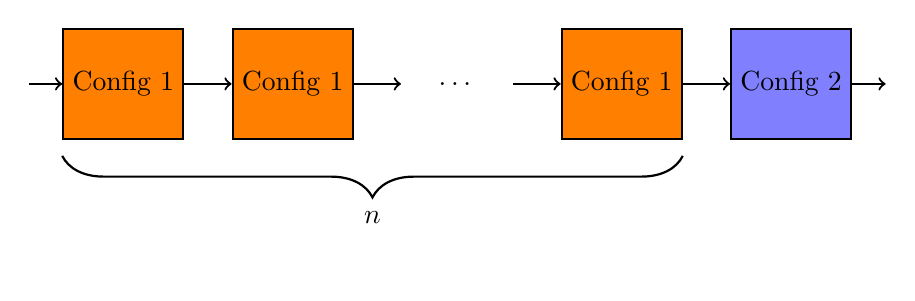
\begin{tikzpicture}[
                node distance=1.2cm and 0.6cm,
                every node/.style={draw, minimum width=1.4cm, minimum height=1.4cm, align=center},
                thick
            ]

            % Define nodes
            \node[fill=orange] (box1) {Config 1};
            \node[right=of box1,fill=orange] (box2) {Config 1};
            \node[right=of box2, style={draw=none}] (box3) {$\dots$};
            \node[right=of box3,fill=orange] (dots) {Config 1};
            \node[right=of dots,fill=blue!50] (boxN) {Config 2};

            % Arrows connecting boxes
            \draw[thick,<-] (box1) -- ++(-1.2,0);
            \draw[thick,->] (box1) -- (box2);
            \draw[thick,->] (box2) -- (box3);
            \draw[thick,->] (box3) -- (dots);
            \draw[thick,->] (dots) -- (boxN);
            \draw[thick,->] (boxN) -- ++(1.2,0);

            % Curly brace underneath the boxes
            \draw[decorate, decoration={brace, amplitude=15pt, mirror}, thick]
            ($(box1.south west) + (0,-0.2)$) -- ($(dots.south east) + (0,-0.2)$)
            node[midway, below=2pt,draw=none] {$n$};


        \end{tikzpicture}
        }
    \end{center}
\end{frame}


\begin{frame}
    \frametitle{Naive Early Stopping}

    \begin{itemize}
        \item Changes to AutoPas are minimal
              \begin{itemize}
                  \item Keep track of best performance seen so far
                  \item \texttt{slowdownFactor} $= \frac{t_{\text{sample}}}{t_{\text{best}}}$
                  \item Call \texttt{retune()} if slowdownFactor exceeds threshold
              \end{itemize}


        \item Hyperparameter: $earlyStoppingFactor$

        \item Which $earlyStoppingFactor$ should be used?
              \begin{itemize}
                  \item $earlyStoppingFactor \rightarrow 1$: Many aborts
                  \item $earlyStoppingFactor \rightarrow \infty$: No early stopping
              \end{itemize}

        \item Empirical evaluation needed
    \end{itemize}
\end{frame}

\begin{frame}{Benchmark: Exploding Liquid + PredictiveTuning}

    \begin{itemize}
        \item Optimal at $earlyStoppingFactor = 5$
        \item From 28.6s to 23.2s
              \begin{itemize}
                  \item[$\rightarrow$] 18.9\% reduction
              \end{itemize}
    \end{itemize}


    \begin{figure}[H]
        \centering

        \includegraphics[width=0.92\columnwidth]{../../data/explodingLiquid/cluster/predictiveTuning/analytics/total_time_average_full_scale.png}


    \end{figure}

\end{frame}


\begin{frame}
    \frametitle{Summary and Future Work}

    \begin{itemize}
        \item AutoPas Library
              \begin{itemize}
                  \item Flexible and optimal N-body simulations
                  \item AutoTuning can cause overhead
              \end{itemize}
        \item (Naive) Early stopping is beneficial
              \begin{itemize}
                  \item Never increased runtime!
                  \item Potential for further improvements
              \end{itemize}
        \item $earlyStoppingFactor$ probably not universal
              \begin{itemize}
                  \item More benchmarks needed!
                  \item Investigate other stopping criteria
              \end{itemize}
    \end{itemize}
\end{frame}


\begin{frame}
    \begin{center}
        \vspace{1cm}
        {\large \textbf{Thank you for your attention!}}

        \vspace{2cm}

        \Huge{Questions?}
    \end{center}
\end{frame}




\begin{frame}[allowframebreaks, noframenumbering]
    \frametitle{References}
    \footnotesize
    \bibliographystyle{apalike}
    \bibliography{literature}
\end{frame}





\end{document}